\documentclass[11pt,a4paper]{article}
\usepackage[top=3cm, bottom=2cm, left=3cm, right=2cm]{geometry}
\usepackage[utf8]{inputenc}
% \usepackage[T1]{fontenc}
\usepackage{amsmath, amsfonts, amssymb}
\usepackage{siunitx}
\usepackage[brazil]{babel}
\usepackage{graphicx}
\usepackage[margin=10pt,font={small, it},labelfont=bf, textfont=it]{caption}
\usepackage[dvipsnames, svgnames]{xcolor}
\DeclareCaptionFont{MediumOrchid}{\color[svgnames]{MediumOrchid}}
\usepackage[pdftex]{hyperref}
\usepackage{natbib}
\bibliographystyle{plainnat}
\bibpunct{[}{]}{,}{s}{}{}
\usepackage{color}
\usepackage{footnote}
\usepackage{setspace}
\usepackage{booktabs}
\usepackage{multirow}
\usepackage{subfigure}
\usepackage{fancyhdr}
\usepackage{leading}
\usepackage{indentfirst}
\usepackage{wrapfig}
\usepackage{mdframed}
\usepackage{etoolbox}
\usepackage[version=4]{mhchem}
\usepackage{enumitem}
\usepackage{caption}
\usepackage{titlesec}

\titleformat{\section}{\LARGE\color{CarnationPink}}{\thesection}{1em}{}
\titleformat{\subsection}{\LARGE\color{CarnationPink}}{\thesubsection}{1em}{}

\DeclareCaptionLabelFormat{figuras}{\textcolor{CarnationPink}{Figura \arabic{figure}}}
\captionsetup[figure]{labelformat=figuras}

\makeatletter
\renewcommand\tagform@[1]{\maketag@@@{\color{CarnationPink}(#1)}}
\makeatother

\renewcommand{\theequation}{Eq. \arabic{equation}}
\renewcommand{\thefigure}{Fig. \arabic{figure}}

\setlist[itemize]{label=\textcolor{CarnationPink}{$\mathbf{\square}$}}

\setlist[enumerate]{label=\textcolor{CarnationPink}{\arabic*.}, align=left}


\newcounter{exemplo}

\NewDocumentEnvironment{exemplo}{ O{} }{%
\allowbreak
\setlength{\parindent}{0pt}
  \begin{mdframed}[
  leftline=true,
  topline=false,
  rightline=false,
  bottomline=false,
  linewidth=2pt,
  linecolor=CarnationPink,
  frametitlerule=false,
  frametitlefont=\Large\bfseries\color{CarnationPink},
  frametitle={\color{CarnationPink}\normalfont\bfseries #1},
  ]
}{%
  \end{mdframed}
}

\setlength{\fboxsep}{10pt}
\setlength{\fboxrule}{1pt}
\usepackage{float}
\renewcommand{\thefootnote}{\alph{footnote}}
\usepackage{url}
\hypersetup{
    colorlinks=true,
    linkcolor=cyan,
    filecolor=cyan,      
    urlcolor=cyan,
    citecolor=cyan,
    pdftitle={Resumos}
}
\pagestyle{fancy}
\fancyhf{}
\renewcommand{\headrulewidth}{0pt}
\rfoot{Página \thepage}

\title{Proteção Radiológica}
\author{Cálculo de Blindagens\nocite{*}}
\date{\textit{Dalila Mendonça}}
\begin{document}
	\maketitle

    \section{Introdução}

    A implementação de um serviço de Radioterapia passa pelas seguintes etapas:

    \begin{enumerate}
        \item Escolha e aquisição dos equipamentos;
        \item Elaboração do projeto de blindagem;
        \item Elaboração do \textcolor{CarnationPink}{\textbf{RPAS} - \textit{Relatório Preliminar de Análise de Segurança}} contendo o Projeto de Blindagem;
        \item Encaminhamento do RPAS para a CNEN (ANSN - Agencia Nacional de Segurança Nuclear) para obter a autorização para a construção;
        \item  Elaboração do \textcolor{CarnationPink}{\textbf{RFAS} - \textit{Relatório Final de Análise de Segurança}} após a conclusão da construção e realização dos testes de aceite. Neste documento está inserido o Plano de Proteção Radiológica (PPR)
    \end{enumerate}

    A elaboração do RPAS é feita pelo Físico SPR (supervisor de proteção radiológica) e a coordenação da construção é feita pelo arquiteto com assistência direta do Físico Médico.

    Uma construção de Radioterapia está integrada à serviços de energia elétrica, iluminação, condicionamento da ventilação e temperatura, fornecimento de água, drenagem, gases medicinais, acabamento e decoração; Todos realizados com ergonomia e segurança.

    \section{Aspectos do Projeto}

        A portaria 1884/1994 do Ministério da Saúde determina que um serviço de Radioterapia deve ter no mínimo:

            \begin{itemize}
                \item 1 consultório indiferenciado com 7.5 m\textsuperscript{2};
                \item 1 sala de preparo e observação dos pacientes com 6.5 m\textsuperscript{2};
                \item 1 Posto de enfermagem com 6 m\textsuperscript{2};
                \item 1 sala de serviços gerais com 6 m\textsuperscript{2};
                \item 1 oficina para confecção de moldes e máscaras com 10 m\textsuperscript{2};
                \item 1 sala para simulador, que pode ser a mesma da braquiterapia, com área e blindagens compatíveis com os equipamentos;
                \item 1 sala de planejamento e Física Médica com 10 m\textsuperscript{2};
                \item 1 sala de terapia para cada equipamento com área e blindagens compatíveis com a máquina;
                \item Sala de espera para pacientes e acompanhantes;
                \item Depósito para material de limpeza;
                \item Sanitários para funcionários;
                \item Vestiário para pacientes;
                \item Sala de utilidades;
                \item Copa;
                \item Câmara Escura;
                \item Sala administrativa;
                \item Depósito de eequipamentos; e 
                \item Áreas para macas e cadeiras.
            \end{itemize}

    \section{Detalhamento Do Projeto}
        
        \begin{itemize}
            \item O Acesso as salas de tratamento devem ser largos para permitir a entrada da máquina, macas e cadeiras;
            \item O Piso deve suportar cargas pesadas;
            \item Deve haver uma porta na entrada das salas de tratamento mesmo que a radiação que chega na porta seja totalmente blindada pelo labirinto;
            \item A porta deve ter blindagem caso o labirinto não tenha tamanho suficiente para blindar a radiação à níveis do publico devido às limitações de tamanho da sala ou quando receber um equipamento com energia maior;
            \item Equipamentos com Beam-Stopper auxiliam na redução das blindagens;
            \item Equipamentos com energias de fótons maiores que 10 MV requerem uma blindagem de nêutrons na porta;
            \item Portas motorizadas devem possuir mecanismo auxiliar para ser utilizado em caso de falhas mecânicas ou elétricas;
            \item A porta deve possuir um mecanismo que assegure que a porta esteja fechada enquanto ocorra a exposição e deve ser possível ser aberta por fora e por dentro;
            \item A blindagem da porta deve ser homogênea e se extender por alguns centímetros além do vão da porta para evitar a existência de frestas;
            \item  São mandatórios mecanismos ``corta-fogo'' e intertravamento elétrico para que não haja exposição com a porta aberta;
            \item O comando deve ser próximo à entrada da porta para que seja mantido à vigilância da entrada pelos técnicos;
            \item Os cabos elétricos devem estar dentro de canaletas construídas no alicerce para correrem facilmente para dentro da sala;
            \item devem ser instalados dutos reservas para cabos, esgoto, água e ar-condicionado;
            \item Os materiais dos dutos devem ser compatíveis com a sua utilização: Para cabos(PVC) e para água (Cobre);
            \item Deve ser fixado na porta o trifólio com as escritas ``Cuidado Radiação'' e os nomes dos responsáveis com seus respectivos telefones para casos de emergência;
            \item É necessário um sinal luminoso que indique quando há presença de radiação (luz vermelha) e quando o equipamento está de prontidão para irradiar (luz verde);
            \item Teleterapia com \textsuperscript{60}Co e Braquiterapia HDR exigem que dentro da sala exista um monitor de área independente que sinalize a exposição à radiação de dentro da sala e no comando;
            \item Devem ser instalados botões de emergência dentro das áreas supervisionadas e das salas de tratamento para serem acionados em casos de exposição acidental;
            \item É necessário a intalação de sistemas de água dentro da sala de tratamento para o resfriamento do acelerador linear; E água para a higienização de mãos e dosimetria;
            \item É necessário a instalação de um sistema de Ar-condicionado;
            \item Pode ser necessária a instalação de gases medicinais para anestesias e recuperação do paciente;
            \item Pisos e recessos devem ser impermeabilizados;
            \item A drenagem do solo deve ser um dos primeiros itens da construção, que exige técnica apurada. Deve-se atentar à hidrografia do solo e a existência de lençóis freaticos. Caso forem superficiais, podem inundar a sala de tratamento em um dia de chuva intensa e causar danos irreparáveis à máquina;
            \item O sistema de ar condicionado deve climatizar adequadamente o ambiente e proporcionar recirculação do ar. Para isto podem ser utilizados:
                \begin{itemize}
                    \item Um sistema central: Nesses casos é indicado a entrada pela barreira da porta, tomando cuidado para evitar a saída de radiação secundária. O duto de entrada deve ser blindado com lâminas de chumbo e/ou absorvedores de nêutrons e deve ser feito de forma que sua entrada seja curva;
                    \item Sistema tipo Split: Sistema cuja canalização é feita com tubos de pequenos diâmetros que entram na sala fazendo curvaturas para eliminar o escape de radiação. Como não possuem recirculador, é necessário o provisionamento da renovação do ar. A melhor rota dentro da sala é moir meio de um teto rebaixado seguindo o labirinto;
                    

                    Obs: Sistemas individuais não são recomendados por exigirem uma grande abertura na blindagem que requer uma blindagem adicional complicada
                \end{itemize}
            \item Caso os lasers sejam embutidos nas paredes blindadas, eles devem ser fixados em placas de aço fundifas no concreto com dimensões de 4 cm de espessura e 2.5 cm de margem extra em relação a caixa do laser;
            \item A visualização do paciente deve ser feita com duas câmeras: uma focada no isocentro e outra dando uma visão panorâmica da sala de tratamento;
            \item Deve ser instalado um dispositivo de comunicação oral que permita a comunicação entre a sala de tratamento e o comando;
            \item Deve existir um mobiliário capaz de armazenar todos os dispositivos utilizados no serviço, como: Acessórios de imobilização; blocos, máscaras, aplicadores de elétrons, etc\dots
            \item Um item importante e muita vezes negligenciado é a instalação de dutos apropriados para a passagem dos cabos de dosimetria. Eles devem sair do comando e atravessar a parede para a sala de tratamento de forma que minimize a radiação secundária e impeça a passagem de radiação primária.
        \end{itemize}

    
    \section{Relatório Preliminar de Análise de Segurança}

        \subsection{Formato e Apresentação}

            Todo processo inicia-se com a abertura de um SCRA (Solicitação de Conceção de Licenças e Autorizações) juntamente com um documento elaborado pelo Titular da Instalação apresentando o serviço e descrevendo resumidamente o objetivo do serviço.

            A elaboração do RPAS deve ser estruturada da seguinte maneira:

            \begin{enumerate}
                \item Devem ser enviadas duas cópias do RPAS contendo o sumário geral, o índice de tópicos e definições de siglas, abreviações, símbolos e termos especiais; Ambos devem ser utilizados de forma consistente;
                \item Deve conter um capítulo exclusivo referente a transporte e rejeitos de materiais radioativos quando for aplicável;
                \item As informações devem ser apresentadas de forma clara e concisa, sempre que possível utilizando tabelas, gráficos, esquemas, diagramas e plantas;
                \item Devem obedecer as seguintes recomendações gráficas:

                    \begin{enumerate}
                        \item Folhas de texto: A4
                        \item Esquemas e Gráficos: A4 (\textit{Podem ser com tamanhos maiores contanto que dobradas não ultrapasse o tamanho A4})
                        \item Plantas: Tamanho A0 ou A1
                            \begin{itemize}
                                \item Escala 1:50 para detalhes;
                                \item Escala 1:100 para planta baixas
                                \item Escala 1:500 para situações
                            \end{itemize}
                    \end{enumerate}

                    As folhas deverão ser dobradas para o tamanho A4 contendo carimbo de identificação com  o endereço do serviço, assinatura e CREA do engenheiro ou arquiteto responsável pela obra. É recomendado ter a assinatura e o RT do SPR, porém não é obrigatório.
            \end{enumerate}

        \subsection{Conteúdo do RPAS}
            
            \begin{enumerate}
                \item \textbf{\textcolor{CarnationPink}{Identificação do Serviço na Folha de Rosto}}
                
                    Deve conter o nome oficial, nome fantasia, endereço, telefone, e-mail, nome e qualificação do titular, registro do Responsável Técnico e seu nome, nome e registro do SPR se ja tiver sido contratado

                \item \textbf{\textcolor{CarnationPink}{Descrição dos Equipamentos Emissores de Radiação}}

                    Fabricante, modelo, tipo, radiações emitidas, energias, técnica isocêntrica ou não, taxa de dose nominal, campo máximo de radiação, fuga máxima pelo cabeçote, transmissão pelo ``beam-Stopper'', ambos parâmetros certificados pelo fabricante. TVL de feixe largo para concreto comum e demais materiais utilizados na blindagem, tanto para feixe primário quanto para radiação de fuga e para a radiação espalhada em todas as energias de fótons.

                \item \textbf{\textcolor{CarnationPink}{Descrição Resumida do Funcionamento do Equipamento}}
                
                    Anexar catálogos 
                
                \item \textbf{\textcolor{CarnationPink}{Apresentação dos Trabalhadores e suas Respectivas Qualificações}}
                
                    Identificar o titular, responsável técnico e seu substituto, SPR e seu substituto, descrevendo suas atribuições, responsabilidades e horários de trabalho; Para os demais funcionários é necessário apenas definir suas atribuições;
                
                \item \textbf{\textcolor{CarnationPink}{Descrição dos Instrumentos de Detecção e Monitoração da Radiação que serão Adquiridos}}
                
                    Deverão ser identificados os monitores de área e os dosímetros clínicos.

                \item \textbf{\textcolor{CarnationPink}{Descrever as Instalações do Serviço}}
                
                    Deverão ser descritas as salas blindadas e as salas de apoio, demonstrando as classificação das áreas como livres, supervisionadas ou controladas. Descrever o laboratório de preparação das fontes para braquiterapia sem afterloading remoto; Descrever as salas de tratamento, simulação, comnandos, salas de espera, de exames, banheiros; Identificar acessos, portas, gaps, overlaps, materiais da parede, tubulações, interlocks, botões de emergência, sinalização de advertência, intercomunicação visual e oral, etc \dots
                
                \item \textbf{\textcolor{CarnationPink}{Plantas da Instalação}}

                    Deverá conter no mínimo 3 plantas:

                    \begin{enumerate}
                        \item \textbf{Planta de Situação:} Contendo a localização do serviço de Radioterapia e do Hospital em relação à vizinhança. Deverá estar em uma escala de 1:200 ou 1:500;
                        \item \textbf{Planta do Serviço de Radioterapia:} Contendo todas as instalações do serviço com suas respectivas identificações, realçando as áreas blindadas. Deverá estar em uma escala de 1:50 ou 1:100;
                        \item \textbf{Prancha Detalhada das Áreas Blindadas:} Contendo a planta e os cortes de elevação lateral e elevação frontal para cada equipamento de radioterapia da instalação. As plantas deverão:

                            \begin{itemize}
                                \item Incluir as dimensões das blindagens e a posição dos pontos de cálculo das blindagens;
                                \item Conter o desenho da máquina e dos dispositivos auxiliares nas suas posições, incluindo o feixe primário em todas as direções;
                                \item Indicar a posição da porta, armários, pia, sistemas hidráulicos, tubulações, etc \dots
                                \item Incluir quadro contendo a identificação da máquina, carga de trabalho, limites de dose; E para cada ponto de cálculo de blindagem deverá ser apresentada a classificação da área, fatores de uso, ocupação e distância.
                                \item Deverá estar em uma escala de 1:20 ou 1:50
                            \end{itemize}
                    \end{enumerate}
            
            \end{enumerate}

    \section{Limites e Definições Para o Cálculo de Blindagens}

        \subsection{Limites Autorizados e Classificação das Áreas}

            As dimensões das blindagens devem ser tais que estejam em conformidade com os limites definidos pela CNEN e pelo princípio de otimização. Primeiro deve ser calculado os valores de espessura da barreira para os limites primários de dose efetiva e na sequência determina-se as espessuras da barreira utilizando o princípio de otimização. As áreas com radiação e as áreas circunvizinhas devem ser classificadas como áreas restritas (aos trabalhadores) e áreas livres (para indivíduos do público).
            

            A CNEN dispensa a demonstração dos cálculos de otimização no RPAS quando o projeto assegura que, em condições normais de operação, as três seguintes condições sejam garantidas simultaneamente:

            \begin{enumerate}
                \item A dose efetiva anual para trabalhadores não  exceda $1 \; mSv$
                \item A dose efetiva anual para indivíduos do grupo crítico não exceda $10 \; \mu Sv$
                \item A dose efetiva coletiva anual não exceda o valor de $1 \; pessoa \cdot Sv$
            \end{enumerate}

            Os limites de dose efetiva para fins de cálculo de blindagem são:

            \begin{itemize}
                \item Para trabalhadores: $20 \; mSv / ano$
                \item Para indivíduos do público: $1 \; mSv/ano$
            \end{itemize}

            Os limites derivados semanais utilizados nos cálculos de blindagem, admitindo o total de 50 semanas em 1 ano são:

            \begin{itemize}
                \item Para trabalhadores: $0.4 \; mSv / semana$
                \item Para indivíduos do público: $0.02 \; mSv/semana$
            \end{itemize}

            Para a determinação das blindagens, deverão ser feitas as seguintes considerações:

            \begin{itemize}
                \item A Sala de tratamento deve ser classificada como área controlada;
                \item As salas de comando devem ser classificadas como salas supervisionadas;
                \item As salas de espera, vestiários e banheiros devem ser classificadas como área livre, pois os pacientes são considerados indivíduos do público quando estão fora da sala de tratamento;
                \item Salas de tratamento anexas à sala em que está sendo feito o cálculo de blindagens é considerada como área livre, pois o paciente presente na sala é considerado como um indivíduo do público para a outra sala de tratamento;
                \item No cálculo de barreira primária não é considerada a atenuação do feixe pelo paciente;
                \item Os cálculos devem sempre assumir uma incidência perpendicular da radiação na parede;
                \item Os valores para a radiação de fuga devem respeitar os limites impostos pela CNEN na norma NN 6.10;
                
                \

                \begin{center}
                    \fcolorbox{cyan}{white}{
                    \begin{minipage}{0.8\textwidth}
                        \centering
                        \textcolor{cyan}{\textbf{Limites de Radiação de Fuga Para Aceleradores Lineares de até 10 MV}}

                        \begin{itemize}
                            \item Não exceda 0.2\% da taxa kerma no ar no seu centro em qualquer ponto de um plano circular com 2 m de raio perpendicular centrado no feixe primário;
                            \item Não exceda 0.5\% da taxa kerma no ar no eixo do feixe primário na distância normal de tratamento, exceto no plano circular acima referido, a 1 m do feixe de elétrons dentro do tubo de aceleração entre a origem e o alvo ou janela de elétrons.
                        \end{itemize}
                    \end{minipage}}
                \end{center}
                
                    \textcolor{CarnationPink}{\textbf{Obs:}} Para fins de cálculos de blindagem, assume uma radiação de fuga de 0.1\% ou 1/100;
                
                \item Recomenda-se que os valores para o fator de ocupação em áreas livres sejam muito conservadores;
                \item A \textbf{\textit{\textcolor{CarnationPink}{Regra das Duas Fontes}}} é utilizada como uma medida conservadora, sempre que os componentes de radiação são somados para definir a espessura da parede; Neste caso é utilizada a TVL e a HVL da radiação mais penetrante.
            \end{itemize}

        \subsection{Parâmetros Utilizados no Cálculo de Blindagens}

            Os parâmetros necessários para o cálculo de blindagens são: \textbf{\textit{Limite de Dose (P), Carga de trabalho (W), Fator Uso (U), Fator Ocupação (T), distância do ponto de cálculo até a fonte ou até o isocentro (d) e Tamanho Máximo do Campo de Radiação (l)}}.

        \subsection*{\textcolor{CarnationPink}{Limite de Dose (P)}}

            Os limites de dose utilizados em cálculo de blindagens estão resumidos na Tabela \ref{tb:limitesDoseCalculoBlindagem}.

            \begin{table}[h]
                \centering
                \caption{Limites de Dose Para Cálculos de Blindagem}
                \label{tb:limitesDoseCalculoBlindagem}
                \begin{tabular}{l  c c}
                    \toprule
                     & \multicolumn{2}{c}{Limites de Dose} \\
                     \addlinespace[6pt]
                     & Indivíduo do Público & IOE \\
                     \cmidrule{2-3}
                     \addlinespace[6pt]
                     Anual &  1 mSv/ano & 20 mSv/ano \\
                     \addlinespace[6pt]
                     Semanal & 0.02 mSv/semana & 0.4 mSv/Semana \\
                     \addlinespace[5pt]
                     \hline
                     \hline
                \end{tabular}
            \end{table}

        \subsection*{\textcolor{CarnationPink}{Carga de Trabalho (W)}}

            É a integral do tempo da taxa de dose absorvida determinada na profundidade de dose máxima a 1 m da fonte. 

            \begin{itemize}
                \item O período de tempo para obter a carga de trabalho é de \textbf{1 semana}.
                \item A unidade de medida para a carga de trabalho é $[W] = Gy/semana$
                \item Uma outra carga de trabalho $W_2$ para uma distância diferente da distância de referência de 1 m da fonte, como ocorre em tratamentos de TBI, é obtida através da lei do inverso quadrado da distância:
                
                    \begin{equation}
                        W_2 = W_1 \left(\frac{1 \; m}{d_2}\right)^2
                    \end{equation}

                \item A carga de trabalho é estimada com base na dose absorvida no isocentro em uma semana, calculada a partir do número médio de pacientes tratados em uma semana e a dose média utilizada nos tratamentos. 
                \item A carga de trabalho relacionada aos controles de qualidade e outras medidas feitas pela física no equipamento deve ser considerada nos cálculos de blindagem. O NCRP 49 indica que a carga de trabalho para o controle de qualidade deve ser: $W_{CQ} = 100 \; Gy/semana$ a 1 m da fonte.
                \item Para feixes com duas energias e feixes de elétrons, é necessário separar a carga de trabalho para cada energia de fótons e normalmente a maior energia que determinará a blindagem necessária.
                \item Para Aceleradores Lineares com duas energias de fótons, é utilizada a carga de trabalho da energia mais alta para fins de blindagem. Porém, em algumas situações, é necessário considerar separadamente as cargas de trabalho para cada qualidade do feixe afim de determinar a espessura da barreira primária e secundária.
                \item Deve-se fornecer uma estimativa altamente conservadora para o número de pacientes tratados por dia, utilizando como base o número de equipamentos, dados históricos e demográficos.
                \item Naqueles equipamentos onde não é possível estimar a carga de trabalho clínica, recomenda-se utilizar o valor de 1000 Gy/semana para aceleradores com energia de até 10 MV e 500 Gy/semana para aceleradores com energias acima de 10 MV.
                \item Em equipamentos que utilizam TBI, a carga de trabalho no isocentro é muito maior que os tratamentos convencionais que utilizam a mesma dose absorvida devido à distância extendida utilizada para este tratamento.
                
                \item Em equipamentos que utilizam a técnica de IMRT, há um aumento da radiação de fuga pelo cabeçote e portanto há um aumento da carga de trabalho para a radiação de fuga.
            \end{itemize}

        \subsection*{\textcolor{CarnationPink}{Fator Uso (U)}}

            É definido como a fração da carga de trabalho do feixe primário que é direcionada para a barreira primária. É um fator que é função do ângulo do gantry e irá depender das geometrias utilizadas nos campos de tratamento. Por exemplo, uma variação de \ang{90} entre os campos descreve uma geometria \textit{4-field box}, e o fator uso para estas angulações pode ser utilizado. Porém, um equipamento que realize mais tratamentos com tangentes para mamas terá uma ângulação oblíqua mais adequada para determinação do fator uso. As Figuras \ref{fig:fatorUso} e \ref{fig:fatorUso2} mostram exemplos de fatores uso recomendados por grandes centros.

            \begin{itemize}
                \item O Fator Uso é dependente das técnicas utilizadas na instalação;
                \item O fator uso pode ser definido para as 4 paredes dos ângulos retos (0°, 90°, 180° e 270°) caso esses sejam os ângulos mais utilizados;
                \item Nos Casos em que são utilizados maioritariamente campos tangentes, as incidências nas angulações oblíquas devem ser analisadas;
                \item Em instalações que realizam procedimentos de TBI deverão considerar um maior fator uso para a parede para onde o feixe é direcionado nesse procedimento.
            \end{itemize}

            \begin{figure}[h]
                \centering
                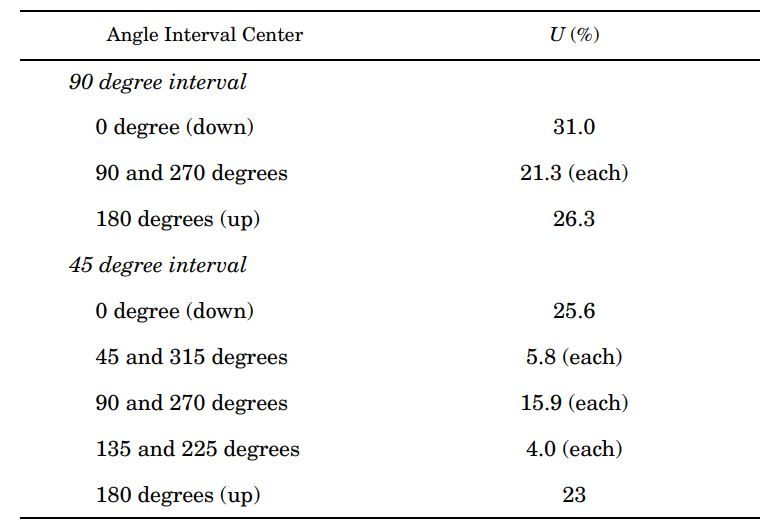
\includegraphics[width=0.8\textwidth]{Imagens/fatorUso.JPG}
                \caption{Exemplo de fator uso para diferentes variações de ângulo de gantry em casos que varia os campos com um intervalo de \ang{90} e \ang{45}.}
                \label{fig:fatorUso}
            \end{figure}

            \begin{figure}[h]
                \centering
                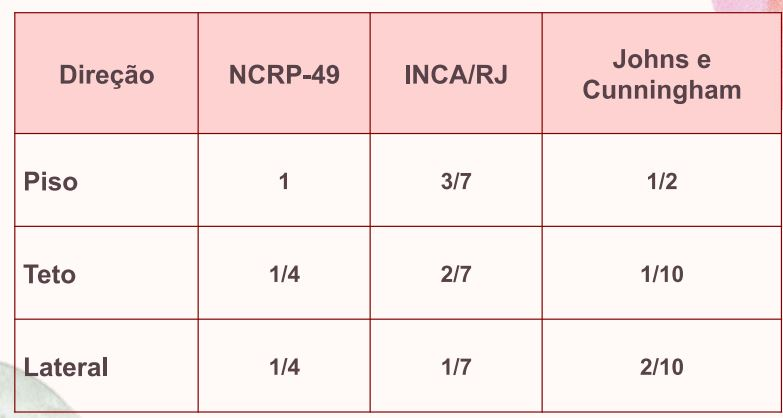
\includegraphics[width=0.8\textwidth]{Imagens/fatorUso2.JPG}
                \caption{Exemplo de fator uso para diferentes variações de ângulo de gantry em casos que varia os campos com um intervalo de \ang{90}.}
                \label{fig:fatorUso2}
            \end{figure}


        \subsection*{\textcolor{CarnationPink}{Fator Ocupação (T)}}

            É a fração média de tempo que o indivíduo com maior tempo de exposição está presente na sala enquanto o feixe está ligado. É determinado através da média semanal de horas trabalhadas avaliadas em um ano. Por exemplo, um fator de ocupação 1/40 diz que o indivíduo com maior exposição permaneceu no local apenas 1 hora por semana.
        
        \subsection{Barreiras de Proteção}

            \begin{wrapfigure}{r}{0.6\textwidth}
                \centering
                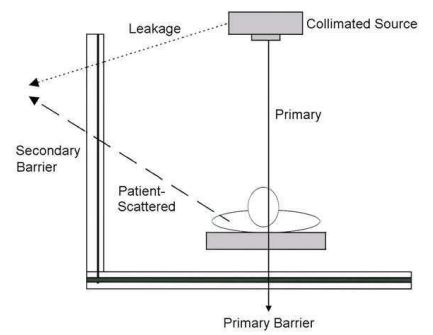
\includegraphics[width=0.58\textwidth]{Imagens/esquemaBarreirasDeProtecao.JPG}
                \caption{Esquema das barreiras de proteção em uma sala de tratamento}
                \label{fig:esquemaBarreirasDeProtecao}
            \end{wrapfigure}

            As barreiras podem ser classificadas como \textit{Barreira Primária ou Barreira Secundária}. A Figura \ref{fig:esquemaBarreirasDeProtecao} apresenta um esquema para a definição das barreiras.

            A \textit{\textcolor{CarnationPink}{Barreira Primária}} é a que protege contra a radiação primária; ou seja, protege contra o feixe útil utilizado nos tratamentos pois está diretamente em frente ao feixe útil do AL. Esta barreira, porém, deve proteger tanto contra o feixe primário quanto o secundário.

            A {\textit{\textcolor{CarnationPink}{Barreira Secundária}}} é aquela barreira que protege contra a radiação secundária, ou seja, a radiação espalhada ou produzida devido a iterações com o paciente e a radiação de fuga do cabeçote. Como a radiação é espalhada em todas as direções, toda a sala terá no mínimo a blindagem para radiação secundária. Algumas ressalvas podem ser feitas, por exemplo no piso, caso esteja localizado em subsolo ou em casos de Skyshine, onde a blindagem poderá ser reduzida.
        
        
        \subsection{Princípios para Diminuição da Exposição}
            
            São 3 os princípios utilizados para diminuir a exposição de um indivíduo à radiação:

            \begin{enumerate}
                \item Aumentando a distância entre o indivíduo e a fonte de radiação;
                \item Limitando o tempo de exposição; e
                \item Adicionando Blindagem entre o indivíduo e a fonte de radiação.
            \end{enumerate}
        
        \subsection{Considerações Para o Cálculo de Blindagens}

        \begin{wrapfigure}{l}{0.5\textwidth}
            \centering
            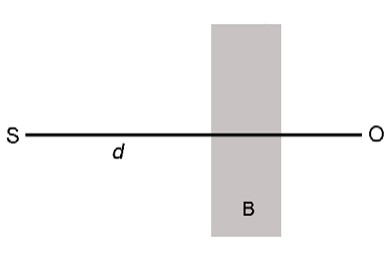
\includegraphics[width=0.5\textwidth]{Imagens/esquemaBasicoDeBlindagem.jpg}
            \caption{Esquema básico de uma blindagem}
            \label{fig:esquemaBasicoDeBlindagem}
        \end{wrapfigure}

        Dado uma fonte de radiação S, localizada a uma distância d de um ponto de análise de dose O (Figura \ref{fig:esquemaBasicoDeBlindagem}), o limite de dose P para esse ponto deve ser respeitado, caso não aconteça, deverá ser adicionada uma barreira B entre S e O para que o feixe seja atenuado até que o limite P seja respeitado.
        
        Para o cálculo de blindagens, alguns aspectos deverão ser considerados, sendo eles:

        \begin{itemize}
            \item Os tipos de radiação que devem ser levados em conta nos cálculos são:
                \begin{itemize}
                     \item A radiação Breamsstrahlung; 
                     \item Os nêutrons;
                     \item A radiação-$\mathrm{\gamma}$
                \end{itemize}
            \end{itemize}
        
            \

            A radiação de Breamsstrahlung acontece no cabeçote do acelerador, na colisão do elétron com o alvo.
            O processo de produção fóton-neutron ($\gamma, n$) ocorre tanto no cabeçote do AL quanto na blindagem da sala.
            Os raios-$\mathrm{\gamma}$ provenientes da captura de nêutrons ocorre apenas na blindagem da sala, sendo um resultado da produção de nêutrons no cabeçote devido aos feixes primários com energia acima da energia de ligação dos nêutrons, que é de aproximadamente 8 MeV para a maior parte dos nuclídeos. De acordo com o NCRP 79 este efeito é mais enunciado para feixes com energia de fótons acima de 10 MeV.
            

            Como ja citado anteriormente, o primeiro passo no cálculo de blindagens é determinar o fator de transmissão B e definir a espessura do material que atende aos limites de dose P, descrevendo os valores da espessura ou a TVL para o material. Para cada ponto e parede, deve ser apresentada as espessuras mínimas para a radiação primária e para a radiação secundária.

            Para os cálculos da porta, deve-se descrever o material da blindagem e levar em consideração os múltiplos espalhamentos no paciente e nas superfícies, descrevendo-os e determinando seus valores e a distância de cada um dos parâmetros avaliados e o percentual de atenuação para a incidência angular.

            Caso não haja ocupação no pavimento superior, serão utilizados os cálculos de espalhamento de radiação no ar para skyshine. Caso contrário, deveram ser calculadas as blindagens não somente para a sala logo acima à sala do acelerador, mas também às salas adjacentes devido à incidências oblíquas.

            Ao final, deverá ser apresentados os cálculos que levaram à determinação das barreiras necessárias para atingir os níveis de dose otimizados dos diferentes pontos de cálculo.

    \section{Cálculos de Blindagem para as Barreiras}

        \subsection{Cálculo de Blindagem Para a Barreira Primária}
            
            A barreira primária deve ser projetada para atenuar o feixe útil de fotons e também atenuar a dose equivalente através da barreira causada por produtos secundários do feixe de fótons, como a radiação-$\mathrm{\gamma}$ e os nêutrons. Em uma barreira adequada, a razão entre a dose equivalente transmitida através da barreira e o limite de dose P para o ponto de análise deve ser menor ou igual a 1.


            O fator de transmissão da barreira primária pode ser obtido através da seguinte relação:

            A intensidade inicial para uma dada parede $I_0$ será a dose total absorvida, considerando o fator uso e o fator ocupação avaliado em um ponto a 0.3m da barreira em análise, portanto a intensidade inicial é definida como:
            
            \begin{equation}
                I_0 = W \cdot U \cdot T
            \end{equation}

            A intensidade que deseja-se alcançar é definida pelo limite \textbf{P} que está a uma distância \textbf{d} da fonte de radiação. Sabendo que o fator W é obtido a uma distância $d_0 = 1 \; m$ da fonte, podemos utilizar a lei do inverso quadrado da distância, para obter uma relação entra a intensidade inicial e a intensidade desejada. 

            
                $$I_0 \cdot d_0^2 = P \cdot d^2$$
            

            Para obter a fração da intensidade de radiação transmitida, basta dividir a intensidade desejada pela intensidade inicial de radiação, o que irá nos fornecer o fator de transmissão da parede.

            
                $$B_{prim} = \frac{P \cdot d^2}{I_0 \cdot d_0^2}$$
            
            Fazendo as devidas substituições, temos que o fator de transmissão para a barreira primária é dado por:

            \begin{equation}
                B_{prim} = \frac{P \cdot d^2}{W \cdot U \cdot T \cdot (1 \; m^2)}
                \label{eq:fatorDeTransmissao}
            \end{equation}

            Onde P é dado em Sv/semana, W é dado em Gy/semana, d é a distância da fonte até o ponto de proteção,  dado em metros e U e T são adimensionais. Portanto o fator de transmissão B\textsubscript{prim} é uma quantidade sem unidade; 

            A espessura da barreira pode ser determinada através das Camadas Deci-Redutoras (TVL's) com base na energia do feixe emitido pelo AL e os tipos de materiais que podem ser utilizados na blindagem. 

            Sabendo que uma TVL reduz a intensidade para 1/10 da intensidade inicial, temos que:
            
            Após 1 TVL:

            $$I_1 = \left(\frac{1}{10}\right)I_0$$

            Após 2 TVL's :

            $$I_2 = \left(\frac{1}{10}\right)I_1 = \left(\frac{1}{10}\right)\left(\frac{1}{10}\right)I_0 = \left(\frac{1}{10}\right)^2 I_0$$

            Após 3 TVL's :

            $$I_3 = \left(\frac{1}{10}\right)I_2 = \left(\frac{1}{10}\right)^3 I_0$$,  

            Portanto, após n TVL's:

            \begin{equation}
                I = \left(\frac{1}{10}\right)^n I_0
                \label{eq:intensidadeAposnTVL}
            \end{equation}
            


            Sabendo que o fator de transmissão é dado por 
            
            $$B = \frac{I}{I_0}$$

            Substituindo este valor na equação \ref{eq:intensidadeAposnTVL}, temos que:

            $$\frac{I}{I_0} = \left(\frac{1}{10}\right)^n $$

            \begin{equation}
                B = \left(\frac{1}{10}\right)^n
                \label{eq:fatorTransmissaoBase10}
            \end{equation}
            

            Aplicando o logaritmo na base 10, temos então:

            $$\log (B) = \log \left(\frac{1}{10}\right)^n $$

            $$\log (B) = n \log \left(\frac{1}{10}\right) $$

            $$\log (B) = n [\log (1) - \log (10) ]$$

           Resolvendo os logaritmos e isolando o numero de TVL's (n), chegamos que:

            $$\log (B) = n (0 - 1)$$
          
            $$ n = - \log(B) $$
           
            Portanto do número de camadas Deci-redutoras necessárias para reduzir a intensidade de radiação à um fator de transmissão B\textsubscript{prim} é dado por:

            \begin{equation}
                n = - \log (B_{prim})
            \end{equation}

            Após atravessar uma certa espessura, ocorre um endurecimento do feixe, pois são filtrados os fótons de energias mais baixas. Portanto há uma mudança no espectro de radiação que penetra a barreira o que faz com que após passar pela primeira TVL, a segunda TVL será mais espessa devido ao endurecimento do feixe. Dados empíricos mostram que a partir da segunda TVL, as espessuras se mantém às mesmas. 

            A espessura da barreira é obtida através da seguinte relação:

            \begin{equation}
                t_{barreira} = TVL_1 + (n - 1)TVL_e
                \label{ eq:espessuraBarreira}
            \end{equation}


            onde, 

            \begin{itemize}
                \item TVL\textsubscript{1} é a primeira camada deci-redutora
                \item TVL\textsubscript{e} é a camada deci-redutora no equilíbrio
            \end{itemize}

            Portanto, se a espessura da barreira for maior que 1 TVL, o fator de transmissão total é dado por:

            Isolando n na equação \ref{ eq:espessuraBarreira}, temos que:

            $$n = 1 + \frac{t - TVL_1}{TVL_e}$$

            Substituindo o valor de n na equação \ref{eq:fatorTransmissaoBase10},

            $$B = \left(\frac{1}{10}\right)^{1 + \frac{t - TVL_1}{TVL_e}}$$

            Obtendo então a relação para o fator de transmissão total:

            \begin{equation}
                B = 10^{-\left\{1 + \left[\frac{t - TVL_1}{TVL_e}\right]\right\}}
            \end{equation}

            Este valor irá representar a verdadeira transmissão da barreira após considerar os valores das camadas deci-redutoras que serão utilizadas na blindagem.

            
            Quando o material utilizado é o concreto, seja ele comum ou denso, a espessura obtida através destes cálculos são suficientes para absorver os fotonêutrons e radiação gama emitida por captura de nêutrons, devido a alta quantidade de hidrogênio presente nesse material e portanto nenhuma barreira adicional é necessária. Porém, ao utilizar outros materiais na barreira primária, algumas considerações especiais precisam ser feitas.

            Embora a técnica de IMRT utilize um alto número de unidades monitoras ou tempo de beam-on, ela utiliza feixes muito estreitos e então a carga de trabalho média sobre qualquer área de 100 cm\textsuperscript{2} na barreira primária é aproximada para as cargas de trabalho padrão;

            \begin{wrapfigure}{r}{0.5\textwidth}
                \centering
                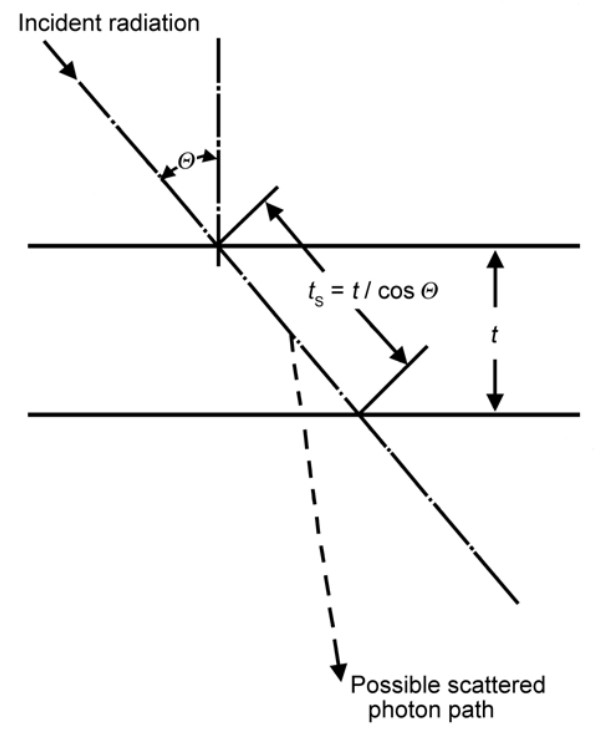
\includegraphics[width=0.4\textwidth]{Imagens/esquemaIncidenciaObliqua.JPG}
                \caption{Esquema de incidência obliqua}
                \label{fig:esquemaIncidenciaObliqua}
            \end{wrapfigure}

            A espessura da barreira primária deve ser calculada para incidências perpendiculares do feixe e deve se manter constante ao longo de toda a largura da barreira. Quando a radiação incide obliquamente na barreia, a espessura requerida será menor que a calculada acima. A diferença dessas espessuras dependem do ângulo de incidência em relação à normal à parede, o material da barreira, a atenuação requerida e a energia da radiação.Se não houvesse espalhamento da radiação no material da barreira, a relação entre a espessura obliqua $t_s$ e a espessura $t$ seria dada por $t_s = t/ \cos \theta$, Figura \ref{fig:esquemaIncidenciaObliqua}. Porém para ângulos grandes ($\theta > \ang{45}$), o fóton espalhado  pode ter um comprimento de caminho $< t_s$ antes de sair da barreira, o que acarretará na necessidade de uma barreira com espessura $> t$. Na maior parte das situações este efeito é pequeno e é tratado como um pequeno aumento na espessura t aproximada. No entanto quando é requerida uma atenuação devido à sua amplitude para ângulos grandes, o aumento na barreira de concreto é de ~ 2 HVL para fótons de baixa energia e de ~1 HVL para fótons de alta energia.

            Os Lasers utilizados no posicionamento devem ser incorporados na blindagem. Esta defasagem na blindagem pode ser em torno de 1 HVL para feixes de alta energia, portando deve ser adicionadas placas de aço ou chumbo com espessura suficiente para fornecer a mesma atenuação da quantidade de blindagem que foi removida para inserção do laser.


        \subsection{Largura do Cinturão Primário}

            O cinturão primário é uma espessura adicionada à barreira secundária na região do feixe primário que é limitada pela largura do cinturão primário; A largura do cinturão primário por sua vez é determinada através do tamanho máximo da diagonal do maior tamanho de campo, somando no mínimo \qty{30}{cm} de cada lado. O cinturão primário pode ser projetado para que a protuberância, relacionada à diferença de espessura entre a barreira primária e a  barreira secundária, fique para dentro da sala de tratamento, ou para fora da sala de tratamento; e dependendo da sua posição, o tamanho máximo do campo utilizado para definir a largura do cinturão primário será diferente. 

            \begin{itemize}
                \item Se a barreira ficar para dentro da sala de tratamento, o tamanho máximo do campo é definido na parte interna da barreira secundária, como mostra a Figura \ref{fig:esquemaCinturaoPrimarioDentroDaSala}. 
                
                    \begin{figure}[h]
                        \centering
                        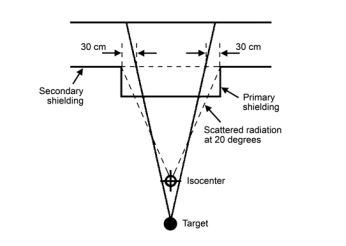
\includegraphics[width=0.4\textwidth]{Imagens/esquemaCinturaoPrimarioDentroDaSala.JPG}
                        \caption{Cinturão primário dentro da sala de tratamento}
                        \label{fig:esquemaCinturaoPrimarioDentroDaSala}
                    \end{figure}


                \item Caso a Barreira seja projetada para ficar fora da sala de tratamento, o tamanho de campo máximo será definido na parte mais externa da barreira primária, como mostra a Figura \ref{fig:esquemaCinturaoPrimarioForaDaSala}
                
                    \begin{figure}[h]
                        \centering
                        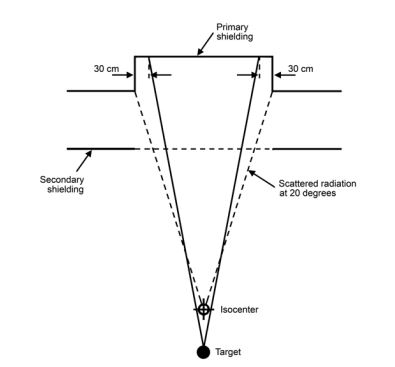
\includegraphics[width=0.4\textwidth]{Imagens/esquemaCinturaoPrimarioForaDaSala.JPG}
                        \caption{Cinturão primário fora da sala de tratamento}
                        \label{fig:esquemaCinturaoPrimarioForaDaSala}
                    \end{figure}

                
                \item Se a Barreira primária é projetada utilizando concreto juntamente com outro material, seja ele aço ou chumbo, a fim de manter toda a parede com a mesma espessura, o tamanho de campo é definido a partir da projeção do campo na superfície mais externa (distal) do chumbo ou aço, como mostra a Figura \ref{fig:esquemaCinturaoPrimarioDoisMateriaisDeBlindagem}.
                    
                    \begin{figure}[h]
                        \centering
                        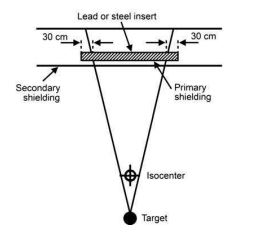
\includegraphics[width=0.4\textwidth]{Imagens/esquemaCinturaoPrimarioDoisMateriaisDeBlindagem.JPG}
                        \caption{Cinturão primário utilizando mais de um material na blindagem}
                        \label{fig:esquemaCinturaoPrimarioDoisMateriaisDeBlindagem}
                    \end{figure}
                
                \item O valor de \qty{30}{cm} só é suficiente caso consiga interceptar a radiação espalhada a \ang{20} a partir do isocentro. 
                
                \item Na maior parte dos aceleradores, o maior tamanho de campo é de \qtyproduct{40 x 40}{cm} na distância Fonte-Superfície (SSD) de \qty{100}{cm}; Com o tamanho máximo da diagonal limitado a aproximadamente \qty{50}{cm} na SSD de \qty{100}{cm}. 
                
                \item A largura da barreira primária é definida no topo da parede primária, que é a região da parede mais longe do isocentro. Esta largura é mantida a mesma para toda a região do cinturão primário.
                
            \end{itemize}

            A maior dimensão do campo no isocentro ocorre na diagonal do campo, quando o colimador está a \ang{45}, como mostra a Figura \ref{fig:maiorDimensaoDoCampo}.

                \begin{figure}[h]
                    \centering
                    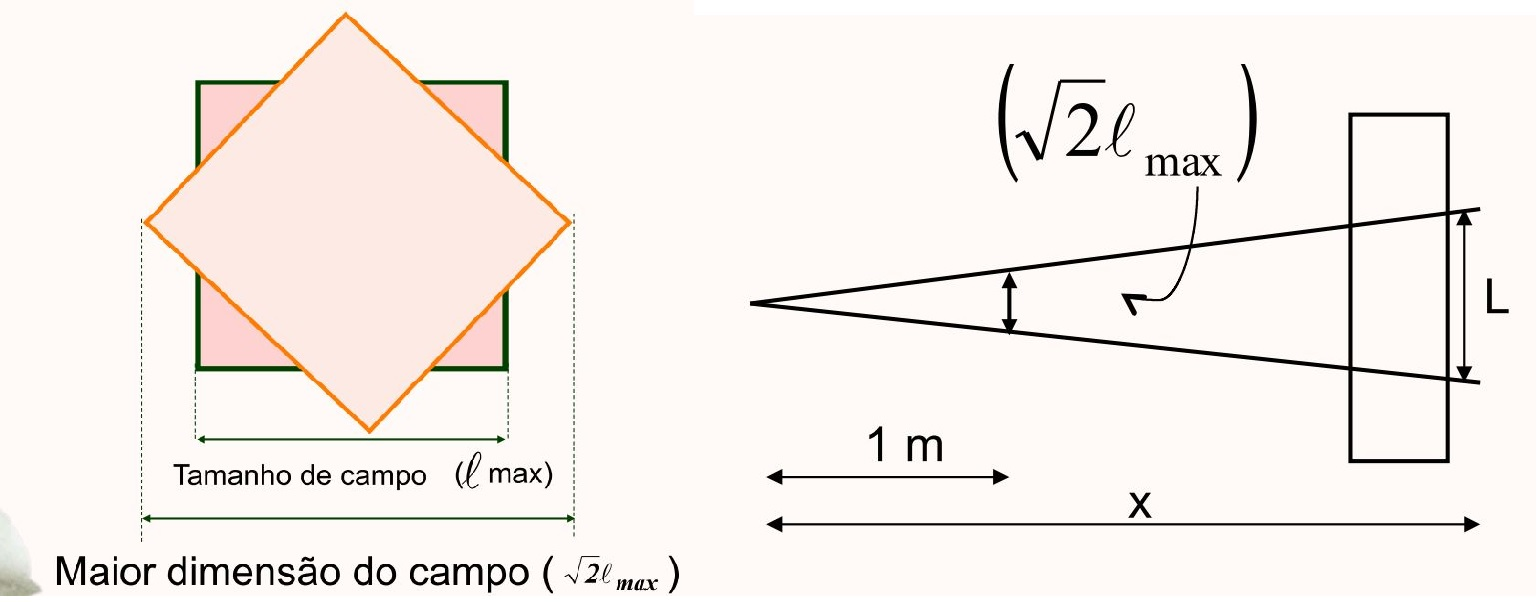
\includegraphics[width=0.9\textwidth]{Imagens/maiorDimensaoDoCampo.JPG}
                    \caption{Maior dimensão do campo}
                    \label{fig:maiorDimensaoDoCampo}
                \end{figure}
            
            Sendo $x$ a distância da fonte até a superfície da barreira e $\ell_{max}$ a largura máxima do campo no isocentro (a 1 metro da fonte), a largura horizontal da barreira primária L é dada por:

                \begin{equation}
                    L = \left(\sqrt{2} \cdot \ell_{max}\right) \cdot x + 0.6
                \end{equation}
                
            É comum que os aceleradores lineares sejam instalados nas salas de tratamento de forma que a rotação do gantry ocorra em um plano ortogonal às barreiras primárias.  No entanto, devido a algumas limitações de espaço, por exemplo, o acelerador pode ser instalado de forma que seu eixo de rotação não esteja ortogonal às barreiras primárias. A Figura \ref{fig:esquemaBarreiraAceleradorAngulado} mostra um acelerador posicionado na sala de forma que seu eixo de rotação está a uma angulação de \ang{45} com as barreiras primárias. 
                
                    \begin{figure}[h]
                        \centering
                        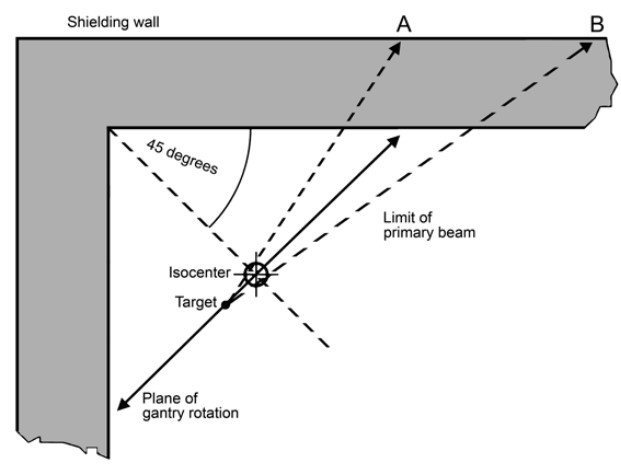
\includegraphics[width=0.4\textwidth]{Imagens/esquemaBarreiraAceleradorAngulado.JPG}
                        \caption{Barreiras para um Acelerador com eixo de rotação do gantry a \ang{45}.}
                        \label{fig:esquemaBarreiraAceleradorAngulado}
                    \end{figure}

                    Nestes casos, deve-se atentar à falta de simetria das posições da extremidades do campo em relação ao eixo central, projetado na barreira primária, uma vez que os fótons que viajam em duas arestas opostas do feixe, embora saiam com a mesma angulação do feixe, atravessarão a blindagem com diferentes angulações de incidência.  
            
        
        \subsection{Barreiras Lamidadas}
            
            São aquelas que utilizam mais de um material para compor a blindagem, como por exemplo, Concreto, Chumbo e Aço.

            O fator de transmissão total para a barreira primária é calculado a partir da multiplicação dos fatores de transmissão para cada material utilizado, ou seja:

            \begin{equation}
                B_{total} = B_{concreto} \cdot B_{chumbo} \cdot B_{aco}
            \end{equation}
            

            Estes cálculos não levam em consideração a atenuação e a produção de fóton-nêutrons ou raios-$\gamma$ emitidos por captura de nêutrons em feixes com energia acima de \qty{10}{MV}. E para estes casos, deve-se atentar à correta disposição dos materiais na blindagem pois a camada de metal pode se tornar uma fonte de fotons-nêutrons, aumentando a exposição além da blindagem. Isto ocorre apenas para a barreira primária, pois a radiação espalhada para além da barreira primária não possui energia suficiente para produzir um fótoneutrôn e a intensidade da radiação de fuga, quando combinada com a seção de choque para produção de fotoneutrôns não produz um número significante de neutrôns nas barreiras secundárias.

            A Dose-equivalente de nêutrons por semana devido a uma barreira laminada quando o colimador está aberto em seu tamanho máximo é obtida pela equação empirica:

            \begin{equation}
                H_n = \frac{D_0 \; R \; F_{max}}{\left(\frac{t_m}{2} + t_2 + 0.3\right)} 
                \left[10^{-\left(\frac{t_1}{TVL_x}\right)}\right]
                \left[10^{-\left(\frac{t_2}{TVL_n}\right)}\right]
            \end{equation}

            Onde: \\
            $H_n$ =  Dose equivalente de nêutrons por semana \\
            $D_0$ =  Dose absorvida de raios-x por semana no isocentro \\
            $R$ = Coeficiente de produção de nêutrons \\
            $F_{max}$ = Área máxima do campo no isocentro \\
            $t_m$ = espessura da camada de metal \\
            $t_1$ = espessura da primeira camada de concreto \\
            $t_2$ = espessura da segunda camada de concreto \\
            $TVL_x$ = camada deci-redutora do concreto para o feixe de raios-x primpario \\
            $TVL_n$ = Camada deci-redutora de concreto para neutrôns \\
            $0.3$ = distancia entre a superfície externa da barreira e o ponto de ocupação.


            \begin{wrapfigure}{l}{0.4\textwidth}
                \centering
                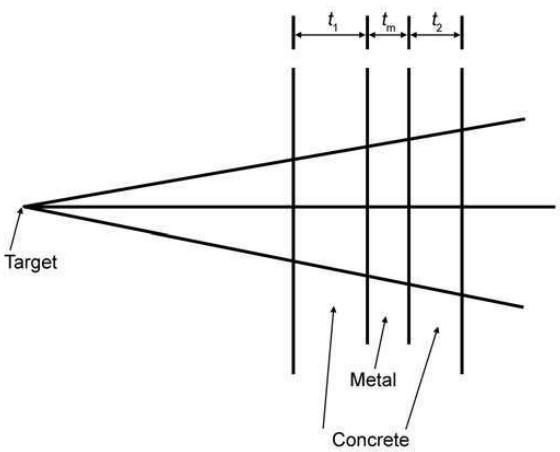
\includegraphics[width=0.36\textwidth]{Imagens/esquemaBarreiraLaminada.JPG}
                \caption{Barreira Laminada}
                \label{fig:esquemaBarreiraLaminada}
            \end{wrapfigure}
            
            \

            A Figura \ref{fig:esquemaBarreiraLaminada} esquematiza a composição de uma barreira laminada. Devido ao processo de produção de nêutrons no metal que subsequentemente interage com o concreto, ocorre a produção de raios-$\gamma$, que são gerados, ou a partir da captura de nêutrons no concreto, ou a partir da desexitação dos núcleos do metal que sofreram interação fotonuclear.

            A dose equivalente total através da barreira $(H_{tot})$ deve então contabilizar a dose equivalente dos nêutrons $(H_na)$ e a dose equivalente para os fótons de raios-x transmitidos $ H_{tr}$ pela parede e dos raios-$\gamma$ produzidos na parede. Baseados em medidas em parades laminadas com energias entre \qtylist{15; 18}{MV} é seguro estabelecer a componente para as radiações x e $\gamma$ sendo 2.7 vezes o valor para a dose equivalente transmitida para a radiação-x, ou seja:

            \begin{equation}
                H_{tot} = H_n + 2.7 H_{tr}
            \end{equation}

            Quando $B_{prim}$ é conhecida, o valor de $H_{tr}$ pode ser obtido através da Equação \ref{eq:fatorDeTransmissao} substituindo $P$ por $H_{tr}$. Se na soma,  $H_{tot} > P$ então o cálculo deve ser iterado para reduzir o valor de $H_{tr}$ até que $H_{tot}$ alcance o limite P definido para a blindagem;

        \subsection{Cálculo de Blindagem para a Barreira Secundária}

            As barreiras secundárias são projetadas de forma quem sejam efetivas na blindagem dos seguintes componentes:

                \begin{enumerate}
                    \item Radiação de fuga do cabeçote;
                    \item Radiação espalhada pelo paciente;
                    \item Radiação espalhada nas paredes; e 
                    \item Radiações secundárias, incluindo fotonêutrons e raios-$\gamma$ produzidos por captura de nêutrons, que devem ser considerados na existência de fótons com energia superior a \qty{10}{MeV} e ao lidar com barreiras finas, como ocorre em portas em um labirinto ou em conduítes 
                \end{enumerate}

            Como a radiação de fuga e a radiação espalhada possuem diferentes energias, os valores da barreira são calculados separadamente para cada uma destas componentes e no final são comparadas para obter a espessura mais recomendada; A Figura \ref{fig:esquemaTransmissaoRadiacaoEspalhadaPaciente} mostra o esquema para cálculos da barreira secundária. 

            \begin{figure}[h]
                \centering
                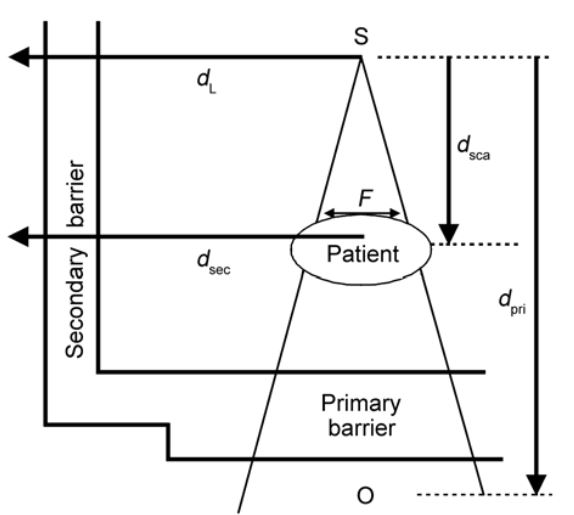
\includegraphics[width=0.6\textwidth]{Imagens/esquemaTransmissaoRadiacaoEspalhadaPaciente.JPG}
                \caption{Barreira Laminada}
                \label{fig:esquemaTransmissaoRadiacaoEspalhadaPaciente}
            \end{figure}

            A transmissão da barreira devido à radiação espelhada pelo paciente é obtida a partir da Equação \ref{eq:BarreiraSecundariaEspalhamentoPaciente}: 

            \begin{equation}
                B_{ps} = \frac{P}{\alpha W T} \; d_{sca}^2 \; d_{sec}^2 \; \frac{400}{F}
                \label{eq:BarreiraSecundariaEspalhamentoPaciente}
            \end{equation}

            E o fator de transmissão para a radiação de fuga é obtido através da Equação \ref{eq:fatorTransmissaoRadiacaoDeFuga}.

                \begin{equation}
                    B_L = \frac{P \; d_L^2}{10^{-3} \; W \; T}
                    \label{eq:fatorTransmissaoRadiacaoDeFuga}
                \end{equation}

            Onde, 


            \begin{itemize}
                \item $B_{ps}$ = É o fator de transmissão devido a radiação espalhada pelo paciente
                
                \item $P$ = É o limite de dose semanal a ser alcançado através da blindagem [\unit{Sv/semana}]
                
                \item $\alpha$ = É a fração de espalhamento ou fração da dose absorvida do feixe primário que é espalhada pelo paciente em um determinado ângulo. É definida como a razão entre a intensidade da radiação espalhada a \qty{1}{m} do objeto espalhador e a intensidade de radiação primária no isocentro.
                
                \item $W$ = É a carga de trabalho semanal [\unit{Gy/semana}] 
                
                \item $T$ = Fator ocupação no ponto localizado a \qty{0.3}{m} da superfície externa da parede
                
                \item $d_{sca}$ = Distância entre o alvo de raios-x e o paciente ou superfície espalhadora [\unit{m}]
                
                \item $d_{sec}$ = É a distância entre a superfície espalhadora e o ponto de proteção [\unit{m}]
                
                \item $400$ = Assume que a fração de espalhamento é normalizada para campos de \qtyproduct{20 x 20}{cm}
                
                \item $F$ = É a área do campo a 1m da fonte medida no centro do paciente [\unit{cm^2}]
                
                \item $d_L$ = É a distância entre o isocentro ao ponto que será protegido [\unit{m}]
                
                \item $10^{-3}$ = Assume que a radiação de fuga pelo cabeçote é de 0.1\% do feixe útil.
            \end{itemize}

            
            \textbf{\textit{\textcolor{CarnationPink}{Obs:}}} O fator uso nas equações da barreira secundária é tomado como sendo igual a 1 para a radiação espalhada pelo paciente. O fator U é uma função do ângulo do gantry. No entanto, se os cálculos são realizados para um ângulo mínimo de espalhamento entre o paciente e o ponto de cálculo e o fator de uso igual a 1 também for utilizado, a espessura da barreira será superestimada devido ao valor para a fração de espalhamento ser conservadoramente alto para pequenos ângulos de espalhamento. 

            \begin{itemize}
                \item Em práticas que utilizam as técnicas de IMRT, a carga de trabalho para a radiação de fuga deve ser alterada.
                
                \item Após determinar o fator de transmissão para radiação espalhada e radiação de fuga, a espessura de material necessária para blindagem é obtida através das TVL's para cada componente.
                
                \item Se a espessura de material necessário para a blindagem é aproximadamente a mesma para cada componente secundaria, como se o espaço ocupado em questão fosse irradiado por duas fontes de intensidade aproximadamente igual,  1 HVL é adicionado à componente que apresentou maior espessura nos cálculos;
                
                \item Se os valores de espessura obtidas pelas componentes secundárias se diferirem em mais de 1 TVL então a espessura mais larga é utilizada;
            \end{itemize}

        
        
            \textbf{\textit{\textcolor{CarnationPink}{Obs:}}} Para fótons, como o fator de qualidade do feixe é igual a 1, a dose equivalente e a dose absorvida são grandezas equivalentes. 
            
        
        \section{Portas e Labirintos}

            Os cálculos para portas e labirintos são separados para Aceleradores Lineares com energia de até \qty{10}{MV} e para Aceleradores Lineares com energias acima de \qty{10}{MV}, pois existem diferenças entre os tipos de radiação secundárias e as fluências produzidas em cada uma dessas faixas de energia.

        \subsection{Aceleradores com Energia de até \qty{10}{MV}}
            

            Um labirinto é desenvolvido para diminuir o nível de radiação na entrada da sala de tratamento sem a necessidade de utilizar uma porta extemamente massiva. E a menos que o labirinto seja muito longo ou que tenha várias voltas, uma blindagem na porta ainda é necessária.

            Para definir a blindagem da porta, é necessário:

            \begin{enumerate}
                \item Determinar a dose equivalente na posição da porta do labirinto avaliada primeiramente para o caso onde o feixe está direcionado perpendicularmente à parede em frente a porta do labirinto;
                \item Utiliza-se uma equação empírica para relacionar a dose equivalente obtida no item anterior à dose equivalente total na porta do labirinto devido aos feixes apontados para às principais direções, 
                \item Determina-se a espessura de material necessária para blindagem afim de reduzir a dose equivalente ao valor do limite P estabelecido.
            \end{enumerate}

            \begin{figure}[h]
                \centering
                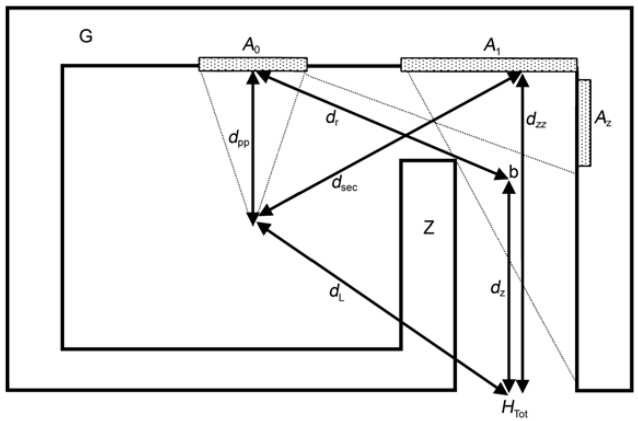
\includegraphics[width=0.6\textwidth]{Imagens/esquemaLabirinto.JPG}
                \caption{Esquematização de um labirinto}
                \label{fig:esquemaLabirinto}
            \end{figure}

            A radiação que alcança a na porta do labirinto é devido aos fótons espalhados nas superfícies da sala e pelo paciente além da radiação de fuga que sai do cabeçote e penetra diretamente o a parede interna do labirinto. As componentes da dose equivalente devido às diferentes radiações que chegam na porta são:

            \begin{itemize}
                \item $H_S$ = Dose equivalente por semana devido ao espalhamento do feixe primário pelas superfícies da sala de tratamento;
                \item $H_{LS}$ = Dose equivalente por semana devido aos fótons provenientes de fuga do cabeçote que são espalhados pelas superfícies da sala;
                \item $H_{ps}$ = Dose equivalente por semana devido ao feixe primário espalhado pelo paciente;
                \item $H_{LT}$ = Dose equivalente da Radiação de fuga que é transmitida diretamente através da parede interna do labirinto.
            \end{itemize}

            A Equação \ref{eq:doseEquivalenteNaPortaDevidoRadiacaoPrimariaEspalhadaNaParede} fornece a componente da radiação primária espalhada pela parede G que chega até a porta, conforme sinalizada na Figura \ref{fig:esquemaLabirinto}.

            \begin{equation}
                H_s = \frac{W \; U_G \; \alpha_0 \; A_0 \; \alpha_z \; A_z}{\left(d_h \; d_r \; d_z\right) ^ 2}
                \label{eq:doseEquivalenteNaPortaDevidoRadiacaoPrimariaEspalhadaNaParede}
            \end{equation}

            Onde:

                \begin{itemize}
                    \item $H_s$ é a dose equivalente por semana na porta do labirinto devido ao espalhamento do feixe primário pela parede G;
                    \item $W$ é a carga de trabalho dada em \unit{Gy \cdot semana^{-1}}
                    \item $U_G$ é o fator de ocupação para a parede G;
                    \item $A_0$ é a area do feixe na primeira superfície de espalhamento dado em \unit{m^2};
                    \item $\alpha_0$ é o coeficiente de reflexão na primeira superfície de espalhamento $A_0$;
                    \item $A_z$ é a segunda superfície de espalhamento, dada como a área da seção transversal da entrada do labirinto, definida pela projeção da área da primeira parede de espalhamento $A_0$ na parede interna da entrada do labirinto;
                    \item $\alpha_z$ é o coeficiente de reflexão para a segunda superfície de espalhamento $A_z$, normalmente assume-se uma energia de 0.5 MeV;
                    \item $d_h$ é a distância perpendicular do alvo até a primeira superfície de espalhamento, igual a $d_{pp}$, que é a distância perpendicular entre o isocentro e a parede somado mais 1m;
                    \item $d_r$ é a distância do centro do feixe na primeira superfície de espalhamento até ao ponto b localizado na linha média do labirinto, passando pela a borda interna do labirinto;
                    \item $d_z$ é a distância da linha central ao longo do labirinto, a partir do ponto b até a porta.
                \end{itemize}
            
            Este cálculo está restrito a uma das duas condições:

                \begin{enumerate}
                    \item A razão entre a altura e a largura do labirinto deve estar entre 1 e 2;
                    \item O valor obtido através da equação : $$\left[\frac{d_z}{\left(altura \times largura\right)^\frac{1}{2}}\right]$$ deve estar entre 2 e 6; Este valor pode não ser alcançados em muitos casos onde o labirinto é projetado de forma que seja mais curto, principalmente devido à limitações de espaço.
                \end{enumerate}
            
            
            A radiação de fuga do cabeçote que sofre apenas um espalhamento pela área $A_1$ da parede G antes de alcançar a porta representa a Dose equivalente obtida através da Equação \ref{eq:doseEquivalenteRadiacaoDeFugaEspalhada}

                \begin{equation}
                    H_{LS} = \frac{L_f \; W_L \; U_G \; \alpha_1 \; A_1}{\left(d_{sec} \; d_{zz}\right)^2}
                    \label{eq:doseEquivalenteRadiacaoDeFugaEspalhada}
                \end{equation}

            Onde:

                \begin{itemize}
                    \item $H_{LS}$ é a dose equivalente por semana na porta do labirinto devido à um único espalhamento da radiação de fuga do cabeçote;
                    \item $L_f$ é a fração da radiação de fuga a \qty{1}{m} da fonte tomada como 1/1000 ou \qty{0.1}{\%};
                    \item $W_L$ É a carga de trabalho para a radiação de fuga dada em \unit{Gy \; semana^{-1}};
                    \item $U_G$ é o fator uso para a parede G;
                    \item $\alpha_1$ coeficiente de reflexão para o espalhamento da radiação de fuga pela a parede G. Toma como base as energias de \qty{1.4}{MeV} para feixes de fótons de \qty{6}{MV} e \qty{1.5}{MeV} para fótons de \qty{10}{MV};
                    \item $A_1$ área da parede G que pode ser vista pela porta do labirinto dada em \unit{m^2};
                    \item $d_{sec}$ é a distância do alvo até a a linha central do labirinto na parede G; Pode ser tomado a partir do isocentro como uma representação da posição média do alvo;
                    \item $d_{zz}$ distância da linha central do labirinto, tomado a partir da parede G vista da porta do labirinto até a porta;
                \end{itemize}
            
            
            A Dose equivalente na porta devido a radiação espalhada pelo paciente é obtida pela Equação \ref{eq:doseEquivalenteRadiacaoEspalhadaPaciente}:

                \begin{equation}
                    H_{ps} = \frac{a(\theta) \; W \; U_G \; \left(\frac{F}{400}\right) \; \alpha_1 \; A_1}{\left(d_{sca} \; d_{sec} \; d_{zz}\right)^2}
                    \label{eq:doseEquivalenteRadiacaoEspalhadaPaciente}
                \end{equation}

            Onde:

                \begin{itemize}
                    \item $H_{ps}$ É a dose equivalente por semana na parede da porta devido a radiação espalhada pelo paciente [\unit{Gy \; semana^{-1}}]
                    \item $a(\theta)$   fração de espalhamento para a radiação espalhada pelo paciente no ângulo $\theta$;
                    \item $W$ Carga de trabalho para o feixe primário;
                    \item $U_G$ Fator uso para a parede G;
                    \item $F$ Área do campo no meio do DAP do paciente a uma distância de 1m da fonte;
                    \item $\alpha_1$ coeficiente de reflexão na parede G para a radiação espalhada pelo paciente; Pode ser obtido para a energia média dos fótons espalhados em vários ângulos pelo paciente, mas, conservativamente, pode ser utilizada a energia de \qty{0.5}{MeV};
                    \item $d_{sca}$ Distância do alvo para o paciente;
                    \item $d_{sec}$ distância do paciente até o ponto central do labirinto na parede G;
                    \item $d_{zz}$ distância da superfície $A_1$ até a porta do labirinto;
                \end{itemize} 
            
            \textbf{\textit{\textcolor{CarnationPink}{Obs:}}} Para energias superiores a 10MV, a contribuição do espalhamento pelo paciente é ignorada uma vez que se torna insignificante quando comparada com a contribuição devido a radiação de fuga e a radiação gama produzida por captura de nêutrons produzidos no labirinto por nêutrons lentos (K aprox \qty{1}{eV}.)

            A dose equivalente na porta devido a radiação de fuga transmitida pela parede Z do labirinto é obtida pela Equação \ref{eq:doseEquivalenteRadiacaoFugaTransmitida}:

                \begin{equation}
                    H_{LT} = \frac{L_f \; W_L \; U_G \; B}{d_L^2}
                    \label{eq:doseEquivalenteRadiacaoFugaTransmitida}
                \end{equation}

            Onde:

                \begin{itemize}
                    \item $H_{LT}$ é a dose equivalente por semana na porta do labirinto devido a radiação de fuga que atravessa a parede interna do labirinto;
                    \item $L_f$ É a razão da radiação de fuga do cabeçote equivalente a $10^{-3}$ o valor do feixe útil;
                    \item $W_L$ É a carga de trabalho para a radiação de fuga; 
                    \item $U_G$ É o fator uso para a parede G;
                    \item $d_L^2$ distância do alvo até o centro da porta do labirinto, atravessando a parede interna do labirinto (Z);
                \end{itemize}
            
            Após obter todas as contribuições para a dose equivalente, quando o gantry direciona o feixe para a parede vista pela porta do labirinto (G). A dose equivalente na porta devido a parede G é obtida através da Equação \ref{eq:doseEquivalenteTotalNaPortaDoLabirintoParaAParedeG}:

                \begin{equation}
                    H_G = f H_S + H_{LS} + H_{PS} + H_{LT}
                    \label{eq:doseEquivalenteTotalNaPortaDoLabirintoParaAParedeG}
                \end{equation}

            Vale notar que a carga de trabalho W é utilizada para determinar H\textsubscript{G} quando o feixe está direcionado para a parede G, ou seja, utiliza W U\textsubscript{G}, e $f$ é a fração do feixe primário transmitido pelo paciente que alcança a parede G. Por exemplo, $f$ tem  o valor de ~0.25 para feixes de \qtyrange{6}{10}{MV}, quando o tamanho de campo é de \qtyproduct{40 x 40}{cm} e é utilizado um \textit{phantom} de \qtyproduct{40 x 40 x 40}{cm}.
                
            A Dose equivalente total é então obtida então considerando as 4 principais direções de incidência do feixe ($\theta = $ \ang{0}, \ang{90}, \ang{180}, \ang{270}).  Quando o fator uso para cada parede é de 1/4, a dose equivalente total na porta é estimada com base na Dose equivalente para a parede G a partir da Equação \ref{eq:doseEquivalenteTotalParaALcomEMenorQue10}:

                \begin{equation}
                     H_{tot} = 2.64 H_G
                    \label{eq:doseEquivalenteTotalParaALcomEMenorQue10}
                \end{equation}
                
            Esta equação deve ser utilizada com atenção para aqueles casos que não respeitem as condições citadas anteriormente: 

                $$1 < \frac{Altura}{Largura} < 2, $$ e
                $$2 < \left[\frac{d_z}{\left(altura \times largura\right)^\frac{1}{2}}\right] < 6$$

            O fator de transmissão necessário para a blindagem da porta é obtido através da Equação \ref{eq:TransmissaoBlindagemPorta}:

                \begin{equation}
                    B_{door} = \frac{P}{H_{tot}}
                    \label{eq:TransmissaoBlindagemPorta}
                \end{equation}
            

            Algumas considerações finais para a determinação da blindagem na porta:
            \begin{enumerate}
                \item Para AL's com energia menor que \qty{10}{MV}, a blindagem da porta é baseada em dados de transmissão de um feixe largo para fótons de \qty{0.2}{MeV}.
                \item Caso a parede interna do labirinto seja muito estreita, o espectro de energia e intensidade de radiação que chega na porta irá aumentar devido ao aumento da radiação de fuga que é emitida por esta parede. Nestes casos a blindagem da porta será determinada somente pela componente $H_{LT}$ e serão utilizados os dados de transmissão para as energias da radiação de fuga; No geral, este não será o caso se a componente $H_{LT}$ for menor que a componente $H_G$;
                \item Em casos onde existem a técnica de TBI, o valor de \qty{2.64}{H_G} pode não ser aplicável; Como a técnica de TBI envolve o tratamento em uma localização diferente do isocentro, os efeitos da radiação espalhada na porta deverão ser considerados. 
            \end{enumerate}
            
        \subsection{Aceleradores com Energia acima de \qty{10}{MV}}
        

            A Figura \ref{fig:esquemaLabirintonêutrons} mostra o esquema de um labirinto para aceleradores de alta energia. A estimativa de dose equivalente devido aos fótons espalhados através do labirinto pode ser determinada através do método utilizado para Aceleradores com até 10 MV, no entanto, uma vez que a energia média dos raios gama de captura para o concreto é de \qty{3.6}{MeV}, uma porta e labirinto que fornece blindagem suficiente para os raios gama de captura será suficiente para os fótons espalhados.

            Para labirintos em Aceleradores de alta energia, quando a distância do Ponto A até o Ponto B, apresentados na Figura \ref{fig:esquemaLabirintonêutrons}, é maior que 2.5 m, o campo de fótons é dominado pelos raios gama de captura e a componente dos fótons espalhados pode ser ignorada. De fato, a dose equivalente dos fótons fora da porta do labirinto apenas muda ligeiramente quando o tamanho de campo formado pelo colimador é ajustado do tamanho máximo para totalmente fechado ou quando o fantoma (objeto espalhador) é removido da frente do feixe. 

             

            \begin{figure}[h]
                \centering
                \includegraphics[width=0.6\textwidth]{Imagens/esquemaLabirintoneutrons.jpg}
                \caption{Esquema de labirinto para Aceleradores Lineares com energia acima de 10 MV}
                \label{fig:esquemaLabirintonêutrons}
            \end{figure}

    \subsubsection{Dose Equivalente dos Fótons Na Porta do Labirinto}

        Para calcular a dose equivalente dos raios gama de captura na porta da sala de tratamento, é utilizado um método descrito por McGinley onde, a dose equivalente $h_{\varphi}$ para os raios gama de captura na entrada externa do labirinto, por unidade de dose de raios-X absorvida no isocentro é dada pela seguinte equação:

            \begin{equation}
                h_{\varphi} = K \varphi_A 10^{-\left(\frac{d_2}{TVD}\right)}
            \end{equation}


        \begin{exemplo}[onde:]
                \textcolor{CarnationPink}{$\mathbf{K}$} é a razão da dose equivalente dos raios gama de captura (Sv) com a fluência total dos nêutrons no ponto A apresentado na Figura \ref{fig:esquemaLabirintonêutrons}. Um valor médio de K igual a \qty{6.9 e{-16}}{Sv \cdot m^2} foi encontrado com base em medidas realizadas em diversos aceleradores.

                \

                \textcolor{CarnationPink}{$\mathbf{\varphi_A}$} é a fluência total de nêutrons (\unit{m^{-2}}) no ponto A por unidade de dose absorvida (\unit{Gy}) dos raios-X no isocentro.

                \

                \textcolor{CarnationPink}{$\mathbf{d_2}$} é a distância do ponto A até a porta (m).

                \

                \textcolor{CarnationPink}{$\mathbf{TVD}$} é a distância deci-redutora, tendo um valor de \qty{\sim 5.4}{m} para raios-X na faixa entre \qtyrange{18}{25}{MV} e um valor de \qty{\sim 3.9}{m} para feixes de fótons de \qty{15}{MV}.
        \end{exemplo}

        A fluência total de nêutrons na entrada interna do labirinto (Ponto A na Figura \ref{fig:esquemaLabirintonêutrons}) por unidade de dose absorvida de raios-X no isocentro pode ser determinada através da seguinte equação:

            \begin{equation}
                \varphi_A = \frac{\beta Q_n}{4 \pi d_1^2} 
                + \frac{5.4 \beta Q_n}{2 \pi S_r} 
                + \frac{1.3 Q_n}{2 \pi S_r}
            \end{equation}

        \begin{exemplo}[onde:]
                O primeiro termo representa a componente dos nêutrons diretos, o segundo termo representa a componente dos nêutrons espalhados e a terceira componente representa os nêutrons térmicos.

                \

                \textcolor{CarnationPink}{$\mathbf{\beta}$} é o fator de transmissão para os nêutrons que penetram a blindagem do cabeçote, tendo o valor igual a 1 para blindagens com chumbo e 0.85 para blindagens com tungstênio.

                \

                \textcolor{CarnationPink}{$\mathbf{d_1}$} é a distância do isocentro até o ponto A (m).

                \

                \textcolor{CarnationPink}{$\mathbf{Q_n}$} é a força da fonte de nêutrons dada em quantidade de nêutrons emitidos pelo cabeçote do acelerador por Gy de dose absorvida de raios-x no isocentro.

                \

                \textcolor{CarnationPink}{$\mathbf{S_r}$} área total de superfície  da sala de tratamento (\unit{m^2})

                \

                \textcolor{CarnationPink}{$\mathbf{1/2\pi}$} nos termos dos nêutrons espalhados e térmicos representa a fração dos nêutrons que entram no labirinto.
        \end{exemplo}

        A dose equivalente semanal $H_{cg}$ (Sv/semana) para os raios gama de captura é dada por:

            \begin{equation}
                H_{cg} = W_L \cdot h_{\varphi}
                \label{eq:doseEquivalenteRaiosGamaCaptura}
            \end{equation}

        \begin{exemplo}[onde:]
            \textcolor{CarnationPink}{$\mathbf{W_L}$} é a carga de trabalho para a radiação de fuga.
        \end{exemplo}

    \subsubsection{Dose Equivalente dos Nêutrons Na Porta do Labirinto}

        Para Aceleradores operando em energias superiores a 10 MV é necessária uma blindagem na porta tanto para fótons quanto para nêutrons. O a dose equivalente de nêutrons na entrada do labirinto varia um pouco, mas não é afetada pela configuração do colimador. Como a máxima fluência de nêutrons é obtida quando os colimadores estão fechados, espera-se que a maioria dos fotonêutrons se originem no cabeçote dos aceleradores. O campo de nêutrons no labirinto também depende do ângulo do gantry e da localização do plano rotação do alvo na sala de tratamento. Foi demonstrado que o nível de nêutrons na porta é máximo quando o ângulo de gantry está alinhado horizontalmente com a direção 3 - 1, indicado na Figura \ref{fig:esquemaLabirintonêutrons}. 

        A dose equivalente dos nêutrons na entrada externa do labirinto pode ser determinada através de diferentes métodos analíticos que utilizam o conceito de distância deci-redutora (TVD) onde a TVD é aproximadamente igual a três vezes a raiz quadrada do produto da altura vezes a largura da abertura e que cada braço adicional na abertura do labirinto diminui a fluência aproximadamente mais três vezes. 

        No \textcolor{CarnationPink}{\textbf{\textit{Método de Kersey}}} a posição efetiva da fonte de nêutrons é definida no isocentro do acelerador e a dose equivalente para os nêutrons ($H_{n,D}$) na entrada externa do labirinto por unidade de dose absorvida de raios-X no isocentro é dada por:

        \begin{equation}
            H_{n,D} = (H_0) \left(\frac{S_0}{S_1}\right) \left(\frac{d_0}{d_1}\right)^2 10^{-\left(\frac{d_2}{5}\right)}
        \end{equation}

        \begin{exemplo}[onde:]
            \textcolor{CarnationPink}{$\mathbf{H_0}$} é a dose equivalente total para os nêutrons, incluindo os componentes direto, espalhado e térmicos na distância $d_0$ (1.41 m) a partir do alvo por unidade de dose absorvida de raios-X no isocentro (\unit{mSv \cdot Gy^{-1}}). Esses valores são encontrados na tabela B.9 no apêndice do NCRP 151.

            \

            \textcolor{CarnationPink}{$\mathbf{S_0}$} é a área da seção transversal da entrada interna do labirinto.

            \

            \textcolor{CarnationPink}{$\mathbf{S_1}$} é a área da seção transversal do labirinto visto pela entrada externa.

            \

            \textcolor{CarnationPink}{$\mathbf{d_1}$} é a distância do isocentro até o ponto na linha central do labirinto a partir do qual o isocentro é visível (A).

            \

            \textcolor{CarnationPink}{$\mathbf{d_2}$} é a distância do ponto A até a entrada do labirinto (Ponto B) no caso de labirintos com apenas 1 curva. Para labirintos com duas curvas, é a distância do ponto A até o Ponto C somado com a distância do ponto C até o Ponto D.

            \

            \textcolor{CarnationPink}{\textbf{Obs:}} neste método, o quociente igual a 5 indica que o labirinto possui uma TVD de 5 m para a atenuaçãod os nêutrons no labirinto. 

        \end{exemplo}

        Medidas experimentais mostraram que a razão entre a dose equivalente para nêutrons calculada com o método de Kersey e a dose equivalente medida diretamente pode variar entre 0.82 até 2.3 em aceleradores com energia de 15 MV até 18 MV e que a TVD é aproximadamente 16\% menor que 5 m e portanto este valor pode ser usado de forma conservadora.

        O \textcolor{CarnationPink}{\textbf{\textit{Método de Kersey Modificado}}} leva em consideração as diferenças experimentais encontradas no método tradicional afim de se obter uma representação mais realística da dose equivalente devido aos nêutrons, dada pela seguinte equação:

        \begin{equation}
            H_{n,D} = 2.4 \times 10^{-15} \varphi_A \sqrt{\frac{S_0}{S_1}}
            \left[1.64 \times 10^{-\left(\frac{d_2}{1.9}\right)} + 10^{-\left(\frac{d_2}{TVD}\right)}\right]
        \end{equation}

        \begin{exemplo}[onde:]
            \textcolor{CarnationPink}{$\mathbf{H_{n,D}}$} é a dose equivalente devido aos nêutrons na entrada do labirinto por unidade de dose absorvida (Gy) de raios-X no isocentro (\unit{Sv \cdot n^{-1} \cdot m^2}).

            \

            \textcolor{CarnationPink}{$\mathbf{\varphi_A}$} é a fluência de nêutrons por unidade de dose absorvida devido aos fótons no isocentro (\unit{m^{-2} \cdot Gy^{-1}}).

            \

            \textcolor{CarnationPink}{$\mathbf{S_0/S_1}$} razão entre a área da seção transversal da entrada interna do labirinto e a área da seção transversal ao longo do labirinto.

            \

            \textcolor{CarnationPink}{$\mathbf{TVD}$} é a distância deci-redutora, dada em metros, que varia com a raiz quadrada a área da seção transversal ao londo do labirinto (\unit{m^2}) $S_1$, ou seja:

                \begin{equation}
                    TVD = 2.06 \sqrt{S_1}
                \end{equation}
        \end{exemplo}

        A dose equivalente semanal $H_n$ (\unit{Sv / semana}) na porta devido aos nêutrons é dada por:

        \begin{equation}
            H_n = W_L \cdot H_{n,D}
            \label{eq:doseEquivalentenêutrons}
        \end{equation}

        \begin{exemplo}[onde:]
            \textcolor{CarnationPink}{$\mathbf{W_L}$} é a carga de trabalho semanal para a radiação de fuga.
        \end{exemplo}

    \subsection{Dose Equivalente Total na Porta do Labirinto}   

        A dose equivalente semanal total $H_W$ na entrada externa do labirinto é dada pela soma de todas as componentes que contribuem para a dose equivalente, ou seja:

        \begin{equation}
            H_W = H_{tot} + H_{cg} + H_{n}
        \end{equation}

        \begin{exemplo}[onde:]
            \textcolor{CarnationPink}{$\mathbf{H_{tot}}$} é a componente relacionada a radiação de fuga e a radiação espalhada, dada pela Equação \ref{eq:doseEquivalenteTotalParaALcomEMenorQue10}.

            \

            \textcolor{CarnationPink}{$\mathbf{H_{cg}}$} é a componente relacionada aos raios gama de captura, dada pela Equação \ref{eq:doseEquivalenteRaiosGamaCaptura}.

            \

            \textcolor{CarnationPink}{$\mathbf{H_n}$} é a componente relacionada aos nêutrons dada pela Equação \ref{eq:doseEquivalentenêutrons}.
        \end{exemplo}

        Para a maior parte dos aceleradores com energia acima de 10 MV, a componente $H_{tot}$ possui uma ordem de grandeza muito menor que a soma de $H_{cg}$ com $H_n$, de forma que esta componente pode ser desprezada.

    \subsection{Blindagem da Porta}

        A blindagem na porta devido a radiação de fuga e a radiação espalhada pode ser obtida com base no fator de transmissão da porta dado pela Equação \ref{eq:TransmissaoBlindagemPorta}. No entanto, em altas energias a componente devido à fuga e espalhamento é relativamente baixa quando comparado às outras componentes que se tornam energéticamente possíveis para maiores energias (nêutrons e raios gama de captura). A energia média para os raios gama de captura é de \qty{3.6}{MeV} e pode alcancar energias da ordem de \qty{10}{MeV} em casos onde os labirintos são muito curtos. Nestes casos pode ser necessário uma TVL de chumbo (equivalente a 6.1 cm). 

        A energia média dos nêutrons na entrada do labirinto é de \qty{\sim 100}{KeV} com uma TVL de polietileno de 4.5 cm. O Polietileno Borado (BPE) (5\% de boro) é apenas um pouco menos eficaz para nêutrons rápidos mas é muito mais eficaz para nêutrons térmicos quando comparado com o polietileno sem o boro.  A TVL para o BPE é de 3.8 cm para nêutrons com energia de 2 MeV e de 1.2 cm para nêutrons térmicos. Portanto, uma recomendação conservadora é utilizar a TVL de 4.5 cm de BPE nos cálculos de blindagem da porta.

        Para as portas onde o comprimento do labirinto seja da ordem de 8 m ou superior, será necessário entre 0.6 cm de chumbo até 1.2 cm de chumbo e entre 2 cm a 4 cm de BPE. Estes elementos deverão ser dispostos tendo uma camada de BPE entre duas camadas de chumbo pois, o chumbo virado para a fonte de nêutrons irpa reduzir a energia dos nêutrons devido a espalhamentos não-elástivos e então tornará o BPE mais efetivo na blindagem dos nêutrons enquanto que a camada externa de chumbo irá atenuar os raios gama de captura emitidos no BPE com energia de 478 KeV. Quando o labirinto é longo o suficiente para atenuar os nêutrons antes que eles cheguem à porta, a camada externa de chumbo não será necessária.

    \section{Procedimentos Especiais}

    \subsection{TBI}

    Em equipamentos que utilizam TBI, a carga de trabalho no isocentro é muito maior que os tratamentos convencionais que utilizam a mesma dose absorvida devido à distância extendida utilizada para este tratamento. A carga de trabalho para o TBI é dada por:
                
    \begin{equation}
        W_{TBI} = D_{TBI} \cdot d_{TBI}^2
    \end{equation}

    \begin{exemplo}[onde:]
        \textcolor{CarnationPink}{$\mathbf{D_{TBI}}$} e a dose absorvida semanal semanal total no tratamento de TBI
        
        \

        \textcolor{CarnationPink}{$\mathbf{d_{TBI}}$} é a distância do isocentro até a distância de tratamento do TBI.
    \end{exemplo}

    Cada carga de trabalho individual é multiplicada pelo fator uso para fins de cálculo de blindagem e o fator uso para o TBI é igual a 1 para a parede onde o paciente ficará an frente para o tratamento e zero para as demais, portanto a carga de trabalho do TBI só será contabilizada para o cálculo da barreira onde ficará na frente. 

    \subsection{IMRT}

        Nos tratamentos de IMRT, incluindo SRS e SBRT, devido ao pequeno tamanho de campo é necessário um número elevado de unidades monitoras que aquele necessário nos tratamentos convencionais com a mesma dose absorvida no isocentro. 

        O Fator IMRT ($C_I$) é a razão entre o número médio de unidades monitoras por uinidade de dose absorvida prescrita necessária para um tratamento de IMRT ($MU_{IMRT}$) e o número médio de unidades monitoras por unidade de dose absorvida prescrita para um tratamento convencional ($MU_{conv}$). 

        Para obter este fator, toma-se uma amostra de i casos de IMRT e calcula-se a média das unidades monitoras necessárias para entregar uma dose prescrita por fração ($D_{pre}$) para estes i casos e deve-se incluir as medidas de QA necessárias para cada caso, calculadas em média sobre o número total de frações de tratamento. Portanto, $MU_{IMRT}$ é dada por:

        \begin{equation}
            MU_{IMRT} = \sum_{i}\frac{MU_i}{(D_{pre})_i}
        \end{equation}
         
        Na sequência, calcula-se o número de MU necessária para entregar a mesma dose absorvida em um fantoma a 10 cm de profundidade na SSD de 100 cm utilizando um campo 10 cm x 10 cm para obter a quantidade $MU_{conv}$ e então obten-se o fator $C_I$, onde:

        \begin{equation}
            C_I = \frac{MU_{IMRT}}{MU_{conv}}
        \end{equation}

        Os valores de $C_I$ variam de 2 até valores superiores a 10.  O aumento no numero de MU para tratamentos de IMRT não aumentam significativamente a carga de trabalho para a barreira primária ou para a componente da radiação espalhada da barreira secundária pois a dose absorvida no isocentro são similares. No entando, a contribuição na carga de trabalho para a radiação de fuga é significativamente maior por um fator tão grande quanto $C_I$ dependendo da fração de pacientes que são tratados com IMRT.

    \subsection{QA}

        Se as medidas de QA forem realizadas rotineiramente durante o horário normal de trabalho, o efeito na carga de trabalho pode não ser insignificante em comparação com a carga de trabalgho do tratamento convencional e o impacto nos requistos de proteção da barreira deve ser avaliado. 

        Se a verificação da dose absorvida de tratamentos de IMRT constituir uma parte significativa das medições de QA, um fator de QA ($C_{QA}$) semelhante ao fator de IMRT ($C_I$) pode ser necessário para considerar o aumento nas unidades monitoras.


    \subsection{Efeito dos Procedimentos Especiais nos Cálculos}

        \begin{itemize}
            \item \textbf{\textcolor{CarnationPink}{Barreira Primária}}
        \end{itemize}

        Para considerar as diferenças nas cargas de trabalho o produto do fator uso pela carga de trabalho é substituido pela soma dos produtos da carga de trabalho pelo fator uso de cada técnica, portanto:


        \begin{equation}
            WU\vert _{prim} = WU\vert _{wall,scat} = W_{conv}U_{conv} + W_{TBI}U_{TBI} + W_{IMRT}U_{IMRT} + W_{QA}U_{QA} + \dots
        \end{equation}

        \begin{exemplo}[onde:]
            \textcolor{CarnationPink}{$\mathbf{ WU\vert _{prim}}$} é o produto da carga de trabalho pelo fator uso para a barreira de radiação primária.

            \


            \textcolor{CarnationPink}{$\mathbf{WU\vert _{wall,scat}}$} é o produto da carga de trabalho pelo fator uso para a barreira de radiação espalhada pela parede.
            
            \

            
            \textcolor{CarnationPink}{$\mathbf{W_x}$} é a carga de trabalho em Gy/semana a 1 m para o tipo de procedimento x;
            
            \

            
            \textcolor{CarnationPink}{$\mathbf{U_X}$} é o fator uso ou fração do tempo que o feixe provavelmente estará incidindo sobre a barreira durante o tipo de procedimento x.
        \end{exemplo}
    
        \begin{itemize}
            \item \textbf{\textcolor{CarnationPink}{Barreira Secundária - Radiação Espalhada pelo Paciente}}
        \end{itemize}

        Neste caso, a carga de trabalho sera dada pela soma das cargas de trabalho para todas as técnicas avaliada no isocentro, ou seja:

        \begin{equation}
            W_{pat scat_{iso}} = W_{conv} + W_{IMRT} + W_{QA} + \dots
        \end{equation}

        Normalmente é utilizado um ângulo de espalhamento de \ang{90} e um fator uso de 1, onde será alcançado um resultado conservador para a blindagem uma vez que o aumento da intensidade para angulos de espalhamento pequenos quando comparados ao angulo de espalhamento de \ang{90} é geralmente compensado por um fator de uso muito pequeno para angulações de gantry que produzem ângulos de espalhamento pequenos.

        Para tratamentos de TBI que são realizados com uma SSD extendida, a radiação espalhada pelo paciente surge de uma localização diferente  do isocentro e portanto os valores de $d_{sca}$ e $d_{sec}$ serão diferentes e portanto a blindagem necessária para a radiação espalhada pelo paciente devido ao TBI deve ser calculada separadamente.

        Se as TVL's necessárias para blindade m das duas componentes da radiação espalhada pelo paciente (convencionel e TBI) diferirem por menos de 1 TVL, a maior TVL é utilizada e é adicionada 1 HVL na blindagem, caso contrário, se a diferença for maior que 1 TVL, a maior TVL é utilizada. 

        \begin{itemize}
            \item \textbf{\textcolor{CarnationPink}{Barreira Secundária - Radiação de Fuga}}
        \end{itemize}


        A carga de trabalho para a radiação de fuga é dada por:

        \begin{equation}
            W_L = W_{conv} + W_{TBI} + C_I W_{IMRT} + C_{QA} W_{QA}
        \end{equation}

        Este valor é utilizada para cálculos de fuga de fótons e produção de nêutrons.

    \subsection{Taxa De Dose Equivalente Média}

        Ao determinar uma barreira, assume-se que a carga de trabalho será uniformemente distribuída ao longo do ano, pontando é razoável projetar uma barreira que atenda ao valor semanal de 1/50 o valor do objetivo anual. Porém, escalas menores do objetivo da blindagem não são apropriadas e podem se tornar incompatíveis com o princípio ALARA. Mais precisamente, o uso de medidas instantâneas de taxa de dose equivalente (IDR) com o acelerador operando com o output máximo não representa propriamente as verdaderias condições de operação. É mais útil se a carga de trabalho e o fator uso forem utilizados em conjunto com a IDR para avaliar a eficácia da barreira. 

        A taxa média de dose equivalente no tempo (TADR) é a taxa média de dose equivalente atenuada pela barreira sob um período de tempo de operação específico, que depende de W e U e pode ser avaliada em dois periodos de tempo de interesse: semana e hora.

        A taxa média de dose equivalente por semana (${R_W}$) é a TADR avaliada em  um local  durante uma semana de trabalho de 40 horas. Para a barreira primária é dada por:

        \begin{equation}
            R_w = \frac{IDR \cdot W_{pri} U_{prim}}{\dot{D}_0}
        \end{equation}

        \begin{exemplo}[onde:]
            \textcolor{CarnationPink}{$\mathbf{R_w}$} é a TADR avaliada em uma semana (\unit{Sv \cdot semana^{-1}})

            \

            \textcolor{CarnationPink}{$\mathbf{IDR}$} é a taxa de dose equivalente instantânea (\unit{Sv \cdot h^{-1}} medido com o equipamento operando com o output de taxa de dose absorvida $\dot{D}_0$). a IDR é determiada a 30 cm além da barreira e para as medições realizadas em aceleradores é calculada a média de 20s a 60 s dependendo do tempo de resposta do instrumento e do ciclo de pulso do acelerador

            \

            \textcolor{CarnationPink}{$\mathbf{\dot{D}_0}$} é o output da taxa de dose absorvida a 1m (\unit{Gy \cdot h^{-1}})

            \

            \textcolor{CarnationPink}{$\mathbf{W_{prim}}$} é a carga de trabalho para a barreira primária (\unit{Gy \cdot semana^{-1}})

            \

            \textcolor{CarnationPink}{$\mathbf{U_{pri}}$} é o fator uso para o local de análise.
        \end{exemplo}

        Para barreiras secundárias, $R_w$ tem contribuição da radiação de fuga e da radiação espalhada pelo paciente, que é obtida através da seguinte equação:

        \begin{equation}
            R_w = \left(IDR_L \frac{W_L}{\dot{D_0}}\right) + \left(IDR_{ps} \frac{W_{ps} U_{ps}}{\dot{D_0}}\right)
        \end{equation}

        \begin{equation}
            IDR_{ps} = IDR_{tot} - IDR_{L}
        \end{equation}

        \begin{exemplo}[onde:]
            \textcolor{CarnationPink}{$\mathbf{IDR_L}$} é a taxa de dose equivalente medida num ponto localizado a 30 cm atrás da barreira secundária na ausência de um fantoma no isocentro.

            \

            \textcolor{CarnationPink}{$\mathbf{IDR_{tot}}$} é a taxa de dose equivalente medida no mesmo ponto na presença do fantoma.

            \

            \textcolor{CarnationPink}{$\mathbf{IDR_{ps}}$} taxa de dose equivalente medida no mesmo ponto devido a radiação espalhada pelo paciente.

        \end{exemplo}


        Alguns protocolos de segurança especificam um limite de taxa média de dose equivalente TADR com vase no valor integrado da taxa de dose equivalente em qualquer hora ($R_h$) para áreas livres. O NRC determina o valor de 0.02 mSv em qualquer hora. 

        O Valor de $R_h$ é derivado com base no número máximo de pacientes que podem ser tratados em qualquer hora considerando o tempo para o setup. Portanto:

        \begin{equation}
            R_h = N_{max} \bar{H}_{pt} = \frac{N_{max} R_w}{\bar{N}_w}
            = \left(\frac{N_{max}}{40 \bar{N}_h}\right)R_W
            = \left(\frac{M}{40}\right)R_w
        \end{equation}



% TODO: Inserir os valores padrão para cada um dos fatores

\bibliography{ref.bib}
\end{document}
